%!TEX root = ../../Paper.tex
\chapter{Trend Stories}
\label{cha:trend-stories}

\section{Happy New Year}
\label{sec:happy-new-year}
Our analysis period covered the time of Christmas and New Year. Figure \ref{fig:christmas-new-year-time-series} shows the behavior of both trends.  

\begin{figure}[H]
  \centering
        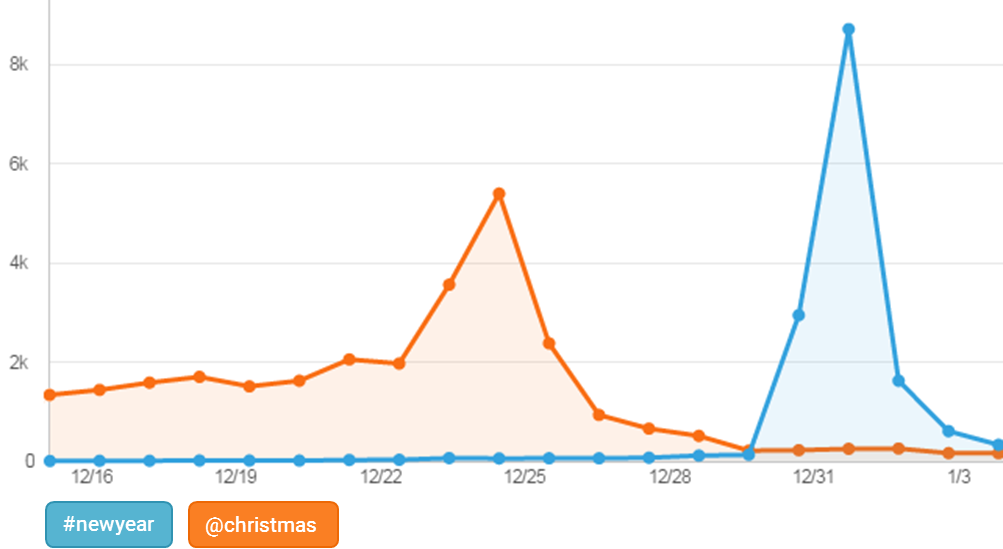
\includegraphics[width=25em]{final_timeseries_newyear}
  \caption[Christmas \& New Year Time Series]{Christmas \& New Year Time Series}
  \label{fig:christmas-new-year-time-series}
  \vspace{-1.3em}
\end{figure}

In the following, we give more insights to the tweets related to the turn of the year due to its rapid increase and the fact that the peak outnumbers the peak during Christmas.. Following hashtags were discovered as being the main used ones: 
\begin{multicols}{3}
\begin{itemize}[label={}]
  \item \#newyear
  \item \#newyearseve
  \item \#nye
  \item \#hny
  \item \#goodbye2014
  \item \#bye2014
  \item \#nye2015
  \item \#midnight
  \item \#ihatenewyears
  \item \#newyearseveproblems
  \item \#newyear2015
  \item \#happynewyear
  \item \#hello2015
  \item \#welcome2015
  \item \#hi2015
  \item \#newyears
\end{itemize}
\fixspacing
\end{multicols}

The word cloud depicted in figure \ref{fig:new-year-word-cloud} illustrates the hashtags and stresses the fact that the identified hashtags are the core ones.

\begin{figure}[H]
  \centering
        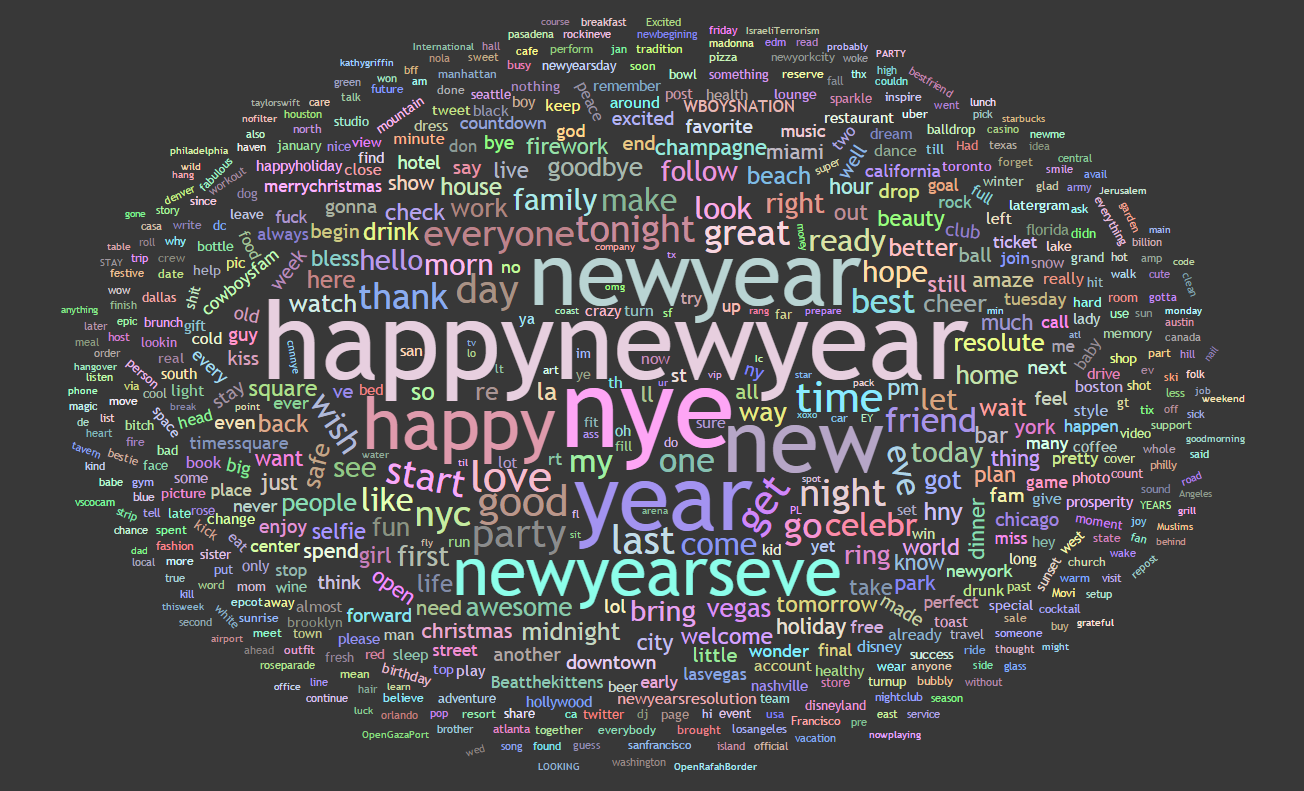
\includegraphics[width=25em]{final_wordcloud_newyear}
  \caption[New Year Word Cloud]{New Year Word Cloud}
  \label{fig:new-year-word-cloud}
  \vspace{-1.3em}
\end{figure}

We chose two different points of time to create the heat maps displayed in figure \ref{fig:new-year-heat-map}.
The left heat map shows the west coast at midnight. The map shows clearly the increase of tweets in the region, especially in Los Angeles. The second map shows the same behavior a few hours before in New York.

\begin{figure}[H]
  \centering
        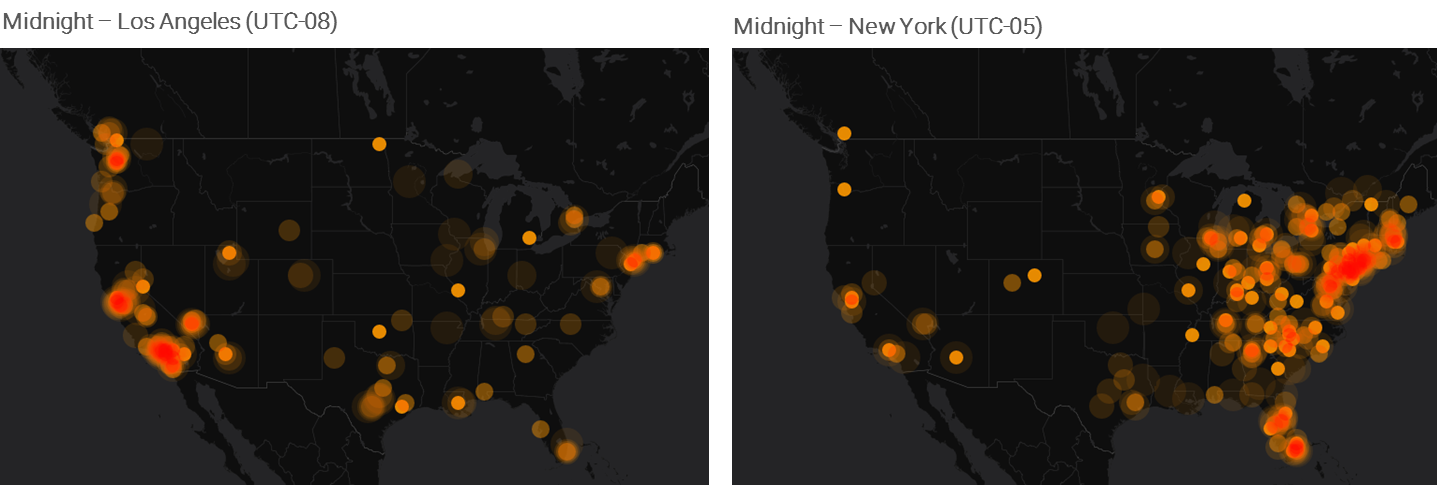
\includegraphics[width=25em]{final_geospatial_newyear}
  \caption[New Year Heat Map]{New Year Heat Map}
  \label{fig:new-year-heat-map}
  \vspace{-1.3em}
\end{figure}

Besides analyzing the locations of the tweets, we analyzed the thoughts of the American people regarding the New Year. More precisely, we focused on the sentiment of the tweets. The results are shown in figure \ref{fig:new-year-sentiment}. Fortunately, the majority of tweets contains positive or at least neutral opinions. Only a small number has a negative attitude.

\begin{figure}[H]
  \centering
        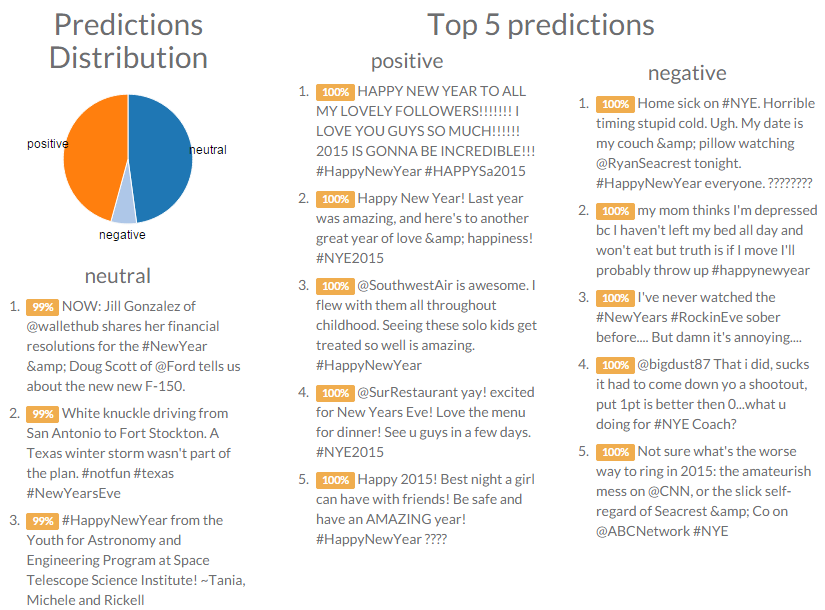
\includegraphics[width=35em]{final_sentiment_newyear}
  \caption[New Year Sentiment]{New Year Sentiment}
  \label{fig:new-year-sentiment}
  \vspace{-1.3em}
\end{figure}


\section{Air Asia Flight Tragedy}
\label{sec:air-asia-flight-tragedy}
\todo{addTOPSY BILD}

On 28th of december a terrible tragedy hit the news: a plane from the Air Asia carrier (QZ8501) crashed into the java sea between Indonesia and Singapore. On board of the flight were 162 people on their way from Surabaya in Indonesia to Changi Airport Singapore. It was around 06:12 local time when the pilot contacted air traffic control to request a change in flight altitude. The pilot wanted to  climb from 9.500 metres up to 11.500 metres in order to prevent being caught by the storm clouds which are typical for that area. Air traffic control gave the permission to do so a few minutes later but could not reach the plane anymore.\cite{bbc2014flight}

Most of the families and relatives of the passengers are still in a deep grief since only 40 victims have been found by now. Experts assume that most passengers are still strapped to their seats in the missing main body of the airplane. As today no survivor has been found and the search is still being continued.\cite{bbc2014air}

When first hearing from the awful tragedy many people thought of the flight 370 from Malaysia Airlines (MH370) which got lost on march 8th. On board of the flight were 239 people including passengers and crew. The search for the plane or its black box have been unsuccessful until today.\cite{nbc2014by}

As shocking this news it we were able to identify an uprise of related tweets on twitter. People were using the following hashtags to discuss this news or to express griefs and sympathy with the families and relatives:

\begin{multicols}{2}
\begin{itemize}[label={}]
	\item \#airasia
	\item \#qz8501
    \item \#prayforairasia
    \item \#prayforqz8501
    \item \#airasia8501
    \item \#mh370
\end{itemize}
\end{multicols}

As mentioned earlier many people connected the crash of Air Asia flight 8501 with the disappearance of the Malaysia Air flight 370 that is why both flight numbers are trending topics. \todo{link to image word cloud air asia!}

\begin{figure}[H]
  \centering
        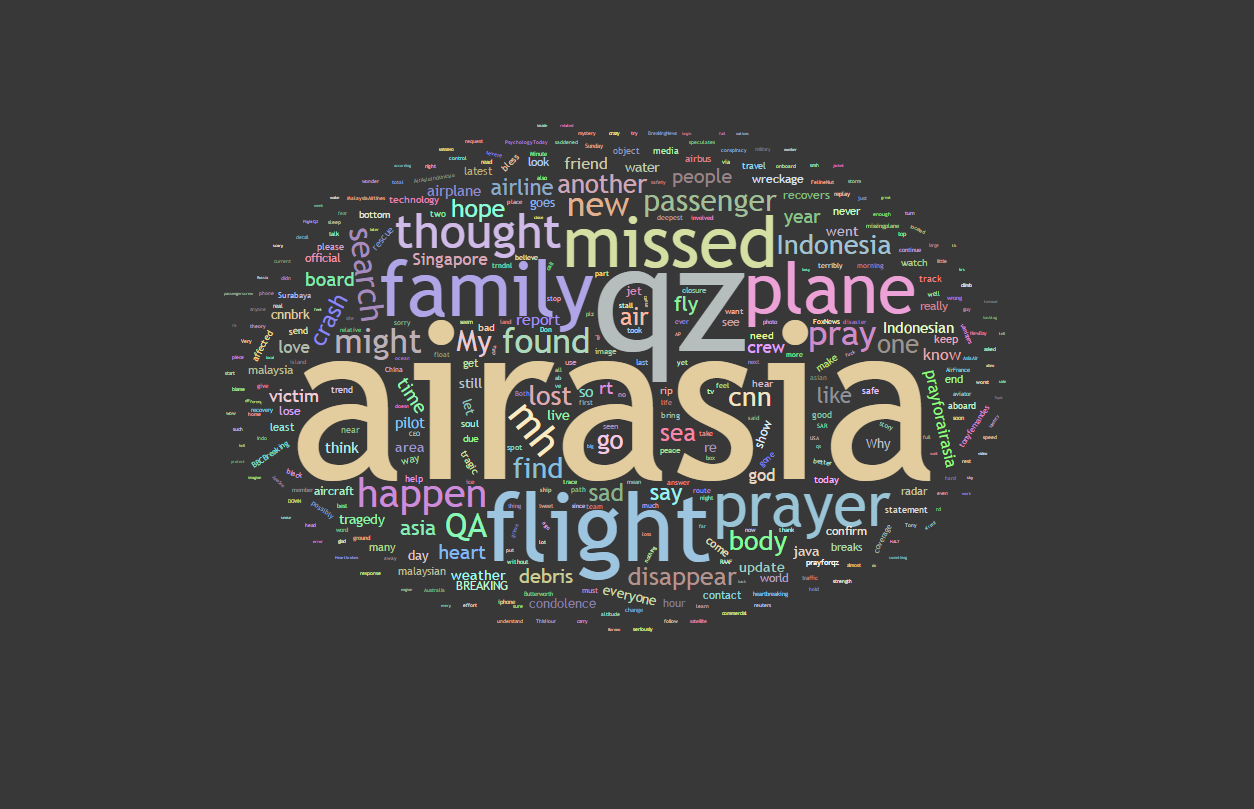
\includegraphics[width=25em]{WordCloud_2_AirAsia}
  \caption[Air Asia Flight Tragedy Word Cloud]{Air Asia Flight Tragedy}
  \label{fig:air-asia-flight-tragedy}
  \vspace{-1.3em}
\end{figure}

The word cloud above depicts the most commonly used words in tweets about the plane crash. A hypothesis based on the wordcloud is that the tweets have two different subjects. One subject is news and tweets are there to inform others about the tragedy and the other subject is emotional and shows condolence to families of the victims.
We extracted all hashtags from our dataset and used LDA for topic modelling in order to further analyze our hypothesis.\todo{link to listing!}

\begin{lstlisting}[caption={[Topic Model for Air Asia Flight Tragedy] Topic Model for Air Asia Flight Tragedy}, label={lst:topic-model-air-asia}, float=h]
	airasia (139) missing (76) flight (55) air (39) indonesia (37) singapore (33) asia (31) °\DNumber°

	airasia (126) missing (60) planes (50) find (39) plane (36) world (20) technology (15) °\DNumber°

	prayers (86) families (81) thoughts (72) airasia (24) crash (14) thought (12) airfrance (8) °\DNumber°

	cnn (13) put (7) speculation (6) ground (6) airasia (6) speed (5) stop (5) °\DNumber°

	airasia (140) found (65) plane (53) sea (51) bodies (49) search (49) debris (40) °\DNumber°

	airasia (146) flight (122) amp (99) happened (87) disappearance (14) malaysia (7) trends (6) °\DNumber°

	airasia (257) families (144) flight (90) passengers (69) prayers (58) amp (47) missing (39) °\DNumber°

	airasia (35) weather (23) flight (17) pilots (13) fly (12) bad (12) path (10) °\DNumber°

	raaf (8) butterworth (8) china (8) australia (5) russia (5) trndnl (5) trending (5)
\end{lstlisting}


We used LDA to model nine different topics showing the 7 most relevant words of each topic. There is an observable difference between reporting tweets (like topic 0, 1, 4 and 7) and emotional tweets (like topic 2 and 6). Topics 3 and 8 stand out from the other, topic 3 is about the famous news network CNN which was one of the first to bring coverage about the crashed plane. Topic 8 on the other hand is about RAAF Butterworth airport in Malaysia, this airport is used by australia and others to coordinate the search for the missing wreckage of the airplane.
This shows that our initial hypothesis is true. There are two different subjects tweeting about the airplane crash of flight QZ8501.


\section{Christmas Network Outage}
\label{sec:christmas-network-outage}
On the 24th of December in 2014, hackers started to attack the Playstation Network and the Microsoft Xbox Live Network. The DDoS attacks brought the networks down for several days. The gamer community was infuriated not to be able to play games during this period of time.\cite{wool2014sony}
After a few days, a hacker group called Lizard Squad claimed credit for the attack.
In the end, the popular german internet entrepreneur Kim Dotcom paid Lizard Squad with vouchers of his web platform Mega \cite{Dotcom2014}. In return, Lizard Squad stopped the attacks letting the gamers play again. Twitter was used by the companies Microsoft and Sony, the gamers, the attackers and Dotcom for discussion, asking for support and negotiating. After the network recovered, Sony announced to give discounts to PSN users. The involved persons and instances and events are reflected in the following list of hashtags and user mentions that were used to tag the related tweets:

\begin{multicols}{3}
\begin{itemize}[label={}]
	\item \#finestsquad
	\item \#lizardpatrol
    \item \#lizardsquad
    \item \#payingfornothing
    \item \#playstationnetwork
    \item \#playstationsucks
    \item \#psn
    \item \#psndown
    \item \#PSNDownTime
    \item \#psnup
    \item \#xboxlivedown
    \item \#xboxsupport
    \item @AskPlayStation
    \item @KimDotcom
    \item @LizardMafia
    \item @MEGAprivacy
    \item @PlayStation
\end{itemize}
  \fixspacing
\end{multicols}

We fetched all tweets containing at least one of the listed hashtags or user mentions and created a word cloud. The resulting word cloud consists of the words used in the fetched tweets.\todo{link to word cloud image!}

\begin{figure}[H]
  \centering
        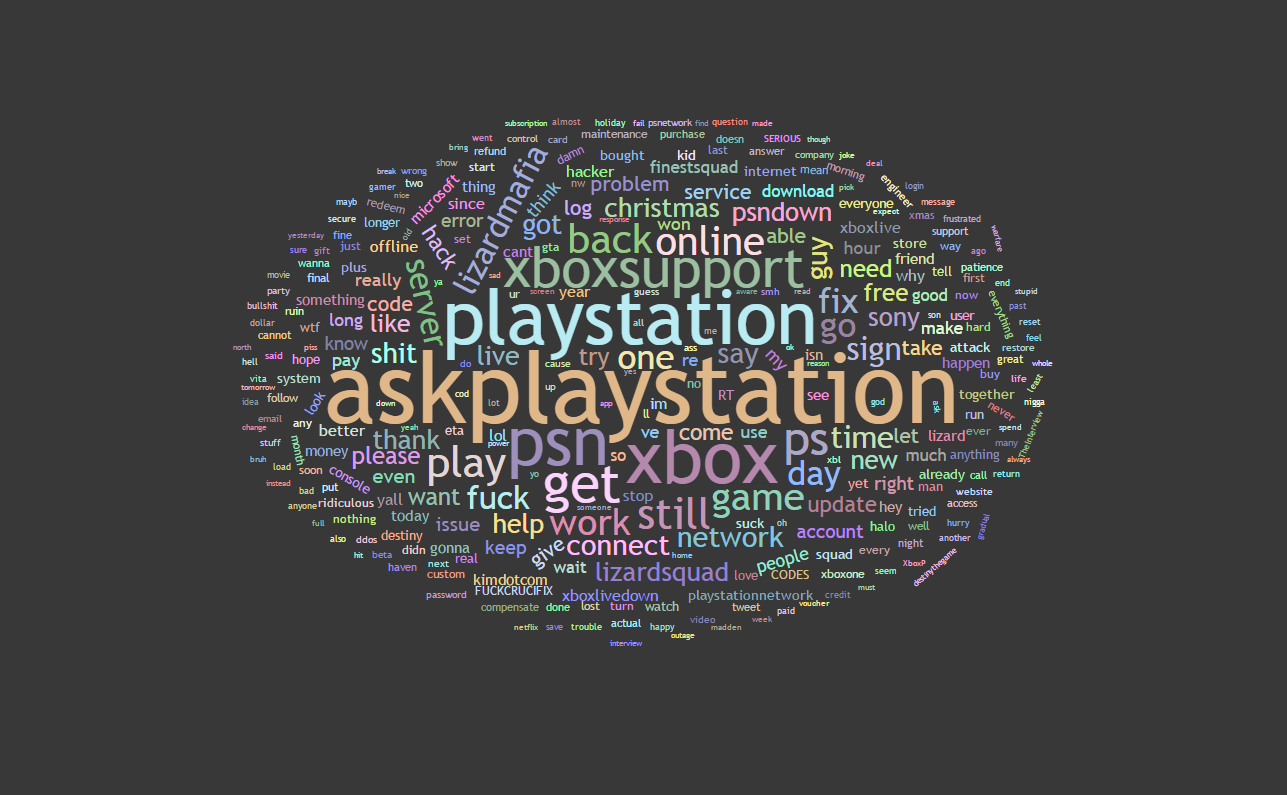
\includegraphics[width=25em]{WordCloud_2_PSNHack}
  \caption[Christmas Network Outage Word Cloud]{Christmas Network Outage Word Cloud}
  \label{fig:christmas-network-outage-word-cloud}
  \vspace{-1.3em}
\end{figure}

The words ‘askplaystation’, ‘playstation’, ‘xbox’, ‘xboxsupport’, ‘psn’ form the core of the cloud.

In the next step, we wanted to find out which of the words in the word cloud are used together most of the time. Therefore, we performed topic modeling on the queried tweets by using LDA.
The identified topics are displayed in the following:

\begin{lstlisting}[caption={[Topic Model for Christmas Network Outage] Topic Model for Christmas Network Outage}, label={lst:topic-model-network}, float=h]
	xbox (101) playstation (50) watch (44) movie (32) fuckcrucifix (31) north (29) korea (27) interview (27) °\DNumber°

	xbox (310) christmas (178) play (81) xboxlivedown (72) live (71) xboxlive (68) xboxsupport (66) day (63) °\DNumber°

	playstation (55) dollar (27) psn (20) company (19) lizardsquad (18) sony (17) billion (16) multi (12) °\DNumber°

	playstation (467) askplaystation (362) shit (279) psn (273) xbox (270) play (246) fix (245) guys (197) °\DNumber°

	fuckcrucifix (204) lizardmafia (172) lizardsquad (125) fuck (116) lizard (108) squad (102) finestsquad (95) stop (94) °\DNumber°

	psn (223) play (217) free (184) games (166) game (153) online (145) xbox (134) codes (93) °\DNumber°

	xbox (95) game (58) warfare (29) controller (24) advanced (24) wait (22) copy (22) party (20) °\DNumber°

	psn (468) back (461) playstation (324) online (246) askplaystation (205) network (173) psndown (89) working (88) °\DNumber°

	halo (61) xbox (45) beta (42) guardians (20) multiplayer (19) xboxsupport (15) live (13) xboxp (12) °\DNumber°

	xbox (250) psn (230) sign (215) connect (143) live (110) error (103) account (93) issues (82) 
\end{lstlisting}

The words that formed the core of the cloud are also dominating the detected topics. Furthermore, the detected topics reflect the real events in a very good way.

Topic 1 covers words indicating a discussion about a connection between the DDoS attack during Christmas and a previous hack against Sony. The earlier attack happened in the end of November, 2014 concerning the movie ‘The Interview’.\cite{bbc2014the}
\todo{Maybe explain a few more details}

The second topic is about the hack affecting the Xbox Live Network. Obviously, a lot of people tweeted to Microsoft's support.
Topic 8 on is similar to topic 2, however, this time the words are concerning Playstation.
Topic 4 covers words about fixing the problem for Playstation as well as Xbox.

Topics 4, 7, 10 cover general terms concerning the hack and the inability to connect to the networks or to play a game.

Topic 5 covers words of tweets that are to or about Lizard Squad. The words indicate that the gamer community was not very amused about the hack.

Topic 3, 6 contain words about the financial impact of such a hack and the claim for redemption for the lost hours of being able to use the networks.

Interestingly, topic 9 contains the word ‘Halo’, which is a game series developed by Microsoft. In another attack in December 2014, parts of the source code of the newest game of the series were stolen. Either the twitter community discussed a possible relation between the two hacks or they were upset not being able to play the current version of the game.\cite{griffin2014unreleased}